\documentclass[tikz,border=2pt,11pt]{standalone}
\usetikzlibrary{arrows.meta}
\usetikzlibrary{calc}
\usetikzlibrary{positioning}
\usepackage{amsmath}
\usepackage{amssymb}
\usepackage{mathrsfs}
\usepackage{xcolor}
\usepackage{tikz}
\newcommand{\C}{\mathbb C}
\newcommand{\R}{\mathbb R}
\newcommand{\Z}{\mathbb Z}
\newcommand{\N}{\mathbb N}
\newcommand{\E}{\mathbb E}
\newcommand{\Prob}{\mathbb P}
\DeclareMathOperator{\diam}{diam}
\DeclareMathOperator{\tr}{tr}
\DeclareMathOperator{\supp}{supp}
\DeclareMathOperator{\dist}{dist}
\DeclareMathOperator{\Var}{Var}
\begin{document}
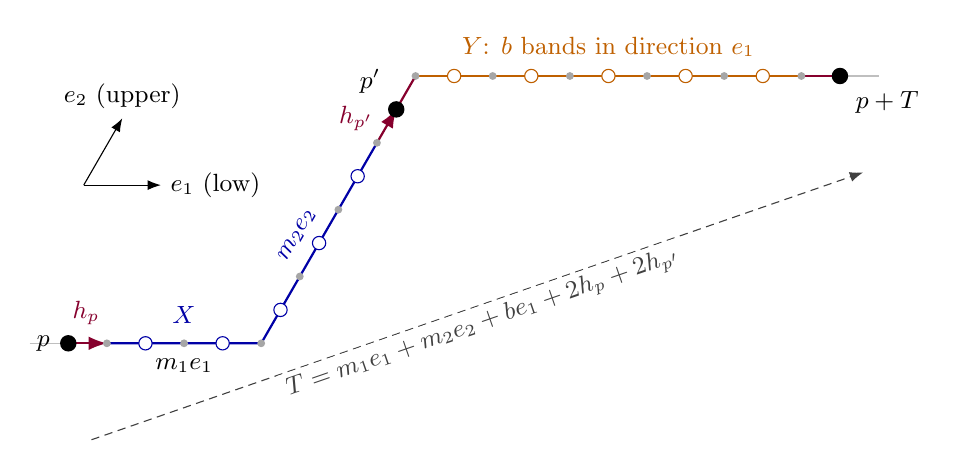
\begin{tikzpicture}[x=0.98cm,y=0.98cm,>=Latex,font=\small,
  ordinary/.style={circle,draw,fill=white,inner sep=1.7pt},
  marked/.style={circle,fill=black,inner sep=2.1pt},
  vertex/.style={circle,fill=black!35,inner sep=1pt}]
 \coordinate (p) at (0,0);
 \coordinate (a) at (0.5,0);
 \coordinate (bend) at (2.5,0);
 \coordinate (c) at (4,{1.5*sqrt(3)});
 \coordinate (pp) at (4.25,{1.75*sqrt(3)});
 \coordinate (d) at (4.5,{2*sqrt(3)});
 \coordinate (e) at (9.5,{2*sqrt(3)});
 \coordinate (pt) at (10,{2*sqrt(3)});

 \draw[thick,blue!65!black] (a)--(bend)--(c);
 \foreach \j in {0,1} {
   \node[ordinary,draw=blue!65!black] at ({1+\j},0) {};
 }
 \foreach \j in {0,1,2} {
   \node[ordinary,draw=blue!65!black]
     at ({2.75+0.5*\j},{(0.25+0.5*\j)*sqrt(3)}) {};
 }
 \node[blue!65!black,above] at (1.5,0.13) {$X$};
 \node[below] at (1.5,-0.08) {$m_1e_1$};
 \node[blue!65!black,rotate=60,above] at (3.15,1.3) {$m_2e_2$};

 \draw[black!25] (-0.5,0)--(p);
 \draw[thick,purple!70!black,->] (p)--(a);
 \draw[thick,purple!70!black,->] (c)--(pp);
 \draw[thick,purple!70!black] (pp)--(d);
 \draw[thick,purple!70!black] (e)--(pt);
 \draw[black!25] (pt)--(10.5,{2*sqrt(3)});
 \node[purple!70!black,above] at (0.23,0.12) {$h_p$};
 \node[purple!70!black,left] at (4.08,{1.68*sqrt(3)}) {$h_{p'}$};

 \draw[thick,orange!75!black] (d)--(e);
 \foreach \j in {0,1,2,3,4} {
   \node[ordinary,draw=orange!75!black]
     at ({5+\j},{2*sqrt(3)}) {};
 }
 \node[orange!75!black,above] at (7,{2*sqrt(3)+0.12})
   {$Y$: $b$ bands in direction $e_1$};

 \foreach \pos in {a,bend,c,d,e} \node[vertex] at (\pos) {};
 \node[vertex] at (1.5,0) {};
 \foreach \j in {1,2} {
   \node[vertex] at ({2.5+0.5*\j},{0.5*sqrt(3)*\j}) {};
 }
 \foreach \j in {1,2,3,4} {
   \node[vertex] at ({4.5+\j},{2*sqrt(3)}) {};
 }
 \node[marked,label={left:$p$}] at (p) {};
 \node[marked,label={above left:$p'$}] at (pp) {};
 \node[marked,label={below right:$p+T$}] at (pt) {};

 \draw[densely dashed,->,black!75]
   (0.3,-1.25)--(10.3,{2*sqrt(3)-1.25})
   node[midway,sloped,below,fill=white,inner sep=2pt]
     {$T=m_1e_1+m_2e_2+be_1+2h_p+2h_{p'}$};

 \begin{scope}[shift={(0.2,2.05)}]
   \draw[->] (0,0)--(1,0) node[right] {$e_1$ (low)};
   \draw[->] (0,0)--(0.5,{sqrt(3)/2})
     node[above] {$e_2$ (upper)};
 \end{scope}
\end{tikzpicture}
\end{document}
